The computing power of integrated circuits has been growing steadily since the dawn of the digital age. In the 20th century, this was mainly achieved
by increasing their clock frequencies to allow for faster executions of the hardware instructions. However, with the beginning of the new millenium,
clock speeds ceased to experience substantial growth rates, mainly due to physical limitations \cite{intelfrequency}. Thus, the focus of circuit
designers shifted to other avenues of performance gains. With Moore's Law still proving to be accurate \cite{mack11mooreslaw}, the number of
transistors fitting onto a single die continues to increase to this day, stimulating the trend towards highly parallelized systems where multiple
processing cores operate side by side \cite[6]{kumar08parallel}. Hence, today's performance gains often stem from a higher level of parallelism
instead of speed increases within single cores.

As the number of processing cores continues to rise, the importance of having an efficient interconnection architecture capable of handling such
highly parallelized systems grows as well. Traditional interconnection architectures employ a global bus that all cores are attached to. However,
buses quickly became a bottleneck for the overall performance \cite[6]{tatas16designingnocs} as their bandwidth is shared by all connected cores. To confront this
scaling problem, novel interconnection approaches were developed, and thus the \textit{Network-on-Chip (\gls{noc})} paradigm was devised
\cites{kumar02networkonchip}{benini02nocparadigm}.

\Glspl{noc} scale significantly better with the number of cores and aim to overcome the drawbacks of traditional buses. However, as the popularity of
\glspl{noc} increases, so does the interest of adversaries to compromise systems
that implement them as their communication backbone. Particularly due to the trend of chip manufacturers integrating a growing amount of third party components, the
threat of the hardware itself being compromised becomes increasingly relevant \cites{ancajas14fortnocs}{sethumadhavan15trustworthyhardware}.

In order to counteract such threats, it is desirable to embed security considerations directly into the design phase of the circuits. In recent
research, numerous approaches to integrate security measures have been pursued\footnote{For an elaborate
discourse on related research, see Chapter \ref{ch:relatedwork}.}. At the TU Dresden Chair of Privacy and Data Security,
\citeauthor{moriam18activeattackers} have explored a method to protect the communications between the cores against adversaries residing in the networking
hardware \cites{moriam15manycorenc}{moriam18activeattackers}. In their approach, network coding was combined with authentication, yielding a
significant increase of their system's resilience to active attackers.

This thesis sets out to expand and improve this approach. Aiming to enhance both performance and security, their scheme is augmented with
encryption and multipath routing, amongst others.

For the TU Dresden, \gls{noc}-related research is of particular importance. In a large-scale, interdisciplinary, and collaborative research center
called \textit{Highly Adaptive and Energy-efficient Computing (\gls{haec})}, a novel approach for massively parallel computing is pursued
\cite{matthiesen17haec}. In this project, a new 3D processor architecture is designed that encompasses numerous compute nodes, each containing
\enquote{thousands of […] cores […] to offer massive intra-node parallelism} \cite[1]{matthiesen17haec}. Hence, an efficient and secure intra-node
interconnection system is crucial to ensure flawless operation of the system. A visualization of their design is given in Figure \vref{fig:haecbox}.

\begin{figure}
    \centering
    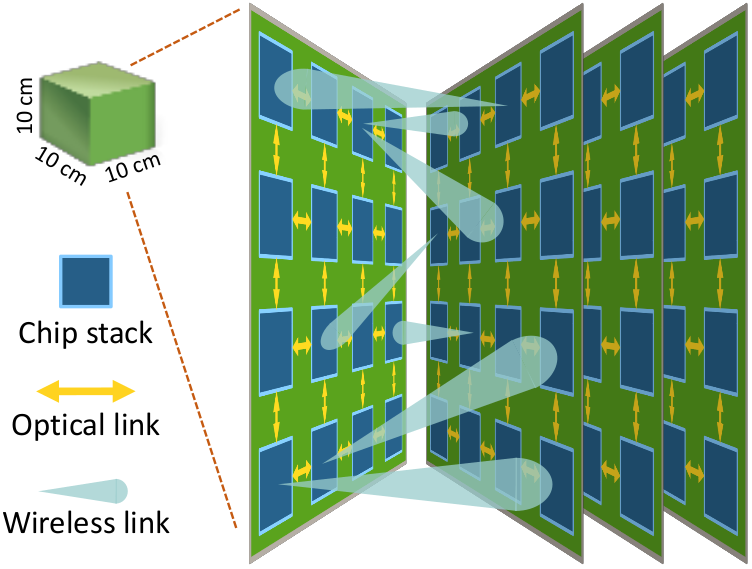
\includegraphics[width=0.4\textwidth]{haecbox}
    \caption[Processor architecture used in the HAEC project]{Processor architecture employed in the \gls{haec} project. Numerous chip stacks are organized
    in compute boards and employ optical and wireless links for their interconnection. Each chip stack is a compute node consisting of multiple
    cores arranged as a 3D mesh, which are interconnected by a wired \gls{noc}. The illustration is taken from the \gls{haec} presentation paper
    \cite[1]{matthiesen17haec}.}
    \label{fig:haecbox}
\end{figure}

The main contributions of this thesis are the conceptualization, implementation, and evaluation of a new approach for secure and efficient
communications in a \gls{noc} that is based upon the foundational work of \citeauthor{moriam18activeattackers}
\cites{moriam15manycorenc}{moriam18activeattackers}. This encompasses the design of an improved communication protocol in multiple variants and its
extensive evaluation through software simulation.

The thesis begins with an explanation of key terms and concepts that are essential for the comprehension of the remainder of this work (Chapter
\ref{ch:fundamentals}). Afterwards, a discourse on related research in the field of \glspl{noc} and their security is provided (Chapter
\ref{ch:relatedwork}). Subsequently, Chapter \ref{ch:overview} gives an overview of the methodologies and courses of action that were employed in this
thesis, followed by an exhaustive and detailed description of the designed communication protocols in Chapter \ref{ch:protocol}. Then, the
implementation of the simulator is presented (Chapter \ref{ch:implementation}), followed by the evaluation of the devised protocols (Chapter
\ref{ch:evaluation}). Finally, the thesis concludes with a summary and an outlook on future work (Chapter \ref{ch:conclusion}).
